%%%%%%%%%%%%%%%%%%%%%%%%%%%%%%%%%%%%%%%%%
% University Assignment Title Page 
% LaTeX Template
% Version 1.0 (27/12/12)
%
% This template has been downloaded from:
% http://www.LaTeXTemplates.com
%
% Original author:
% WikiBooks (http://en.wikibooks.org/wiki/LaTeX/Title_Creation)
%
% License:
% CC BY-NC-SA 3.0 (http://creativecommons.org/licenses/by-nc-sa/3.0/)
% 
% Instructions for using this template:
% This title page is capable of being compiled as is. This is not useful for 
% including it in another document. To do this, you have two options: 
%
% 1) Copy/paste everything between \begin{document} and \end{document} 
% starting at \begin{titlepage} and paste this into another LaTeX file where you 
% want your title page.
% OR
% 2) Remove everything outside the \begin{titlepage} and \end{titlepage} and 
% move this file to the same directory as the LaTeX file you wish to add it to. 
% Then add \input{./title_page_1.tex} to your LaTeX file where you want your
% title page.
%
%%%%%%%%%%%%%%%%%%%%%%%%%%%%%%%%%%%%%%%%%

\documentclass[12pt,a4paper]{article}
\usepackage[english]{babel}
\usepackage[utf8x]{inputenc}
\usepackage{amsmath}
\usepackage{graphicx}
\usepackage[colorinlistoftodos]{todonotes}

\begin{document}

\begin{titlepage}

\newcommand{\HRule}{\rule{\linewidth}{0.5mm}}

\center

\textsc{\LARGE Coursera}\\
\textsc{\large The Hong Kong University of Science and Technology}\\[1cm]
\textsc{\Large Full Stack Web Development Specialization}\\[0.5cm]
\textsc{\large Capstone Project}\\[0.5cm]

\HRule \\[0.4cm]

\includegraphics[width=.5\paperwidth]{mymovies.png}
\HRule \\[1cm]
 

\begin{minipage}{0.4\textwidth}
\begin{flushleft} \large
\emph{Author:}\\
Tiago \textsc{Justino}
\end{flushleft}
\end{minipage}
~
\begin{minipage}{0.4\textwidth}
\begin{flushright} \large
\emph{Supervisor:} \\
Jogesh \textsc{Muppala}
\end{flushright}
\end{minipage}\\[1cm]


{\large \today}\\[1cm]

\vfill

\includegraphics[width=.2\paperwidth]{coursera.png}
\hspace{2cm}

\includegraphics[width=.2\paperwidth]{hkust.png}

\end{titlepage}
%----------------------------------------------------------------------------------------

\begin{abstract}
Your abstract.
\end{abstract}
\newpage

\section{Introduction}

Cinema fans. - ???

A brief introduction to your website/application idea. State the goals of the
project.

MyMovies is a website for keeping track of movies you've watched, want to
watch and don't want to watch. It leverages the IMDB database by allowing the
user to Add custom information, e.g., rating and comments.

The values / benefits (tangible and intangible) this application can bring to a
company/organization/end-user.

Tracking the movie watching habits of the user will help the cinema industry
on targeting its customer more precisely.

\section{Expected List of Features}

\begin{itemize}
  \item Register / Login with or without Facebook.
  \item Add friends (they need to accept your request)
  \item Follow other users (friends are followed by default, but you can
    unfollow a friend without unfriending them)
  \item Mark a movie as watching, watched, want to watch, don't want to watch.
  \item Movies marked as watched can be rated, favorited and commented.
  \item Movies marked as watching are automatically marked as watched after the
    movie duration (known from imdb api).
  \item When marking a movie as watching or watched the user can mark a friend
    in "watching with"
  \item The user can add a date (day, month or year) for movies watched in the
    past. Date is not mandatory.
  \item A movie can be marked as watched more than once.
  \item There will be a timeline where the user can see the activities of whom
    they follow.
  \item A user can like or comment friend's activities.
  \item A comment (or part of it) can be marked as spoiler.
  \item Comments marked as spoiler appear with a warning message on a user
    timeline if they haven't watched that movie.
  \item groups
\end{itemize}

future work

\begin{itemize}
  \item add location to movies marked as watching / watched
  \item recommend movies based on:
    \begin{itemize}
      \item previous watched movies
      \item movies they want to watch
      \item friend's activities
      \item likes
    \end{itemize}
  \item recommend near movie theaters for movies they want to watch
  \item search movie streaming services for movies they want to watch and check
    prices.
  \item allow the user to register movie streaming services they subscribe and
    search on them for movies they want to watch
\end{itemize}

A brief list of features that you expect your application to support.

Brief justifications for including these features.

\section{Market Survey}

filmow.com already implements a similar idea.

Do a survey of the Web and Apple Store and Google Play Store to find about five
web sites and/or applications that might have similar ideas as yours.

Briefly compare the features of these applications with your application idea.

\section{References}

Give references to any material / websites / books etc. relevant to your
application idea

Give the links to the websites and applications on the Apple Store and Google
Play Store relevant to your idea, that you listed in the section above.

%\label{sec:examples}
%
%\todo{Here's a comment in the margin!}
%\todo[inline, color=green!40]{This is an inline comment.}
%
%\begin{figure}
%\centering
%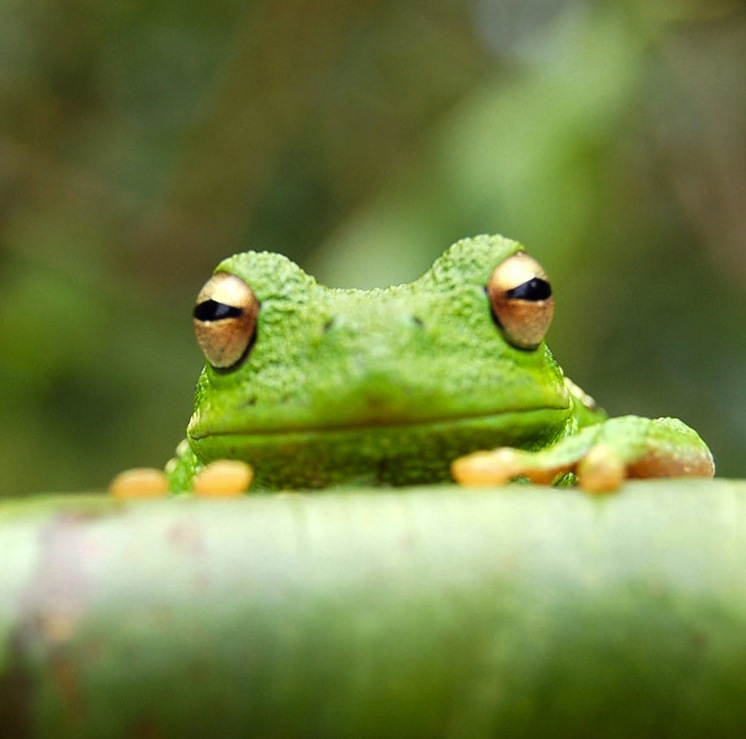
\includegraphics[width=0.5\textwidth]{frog.jpg}
%\caption{\label{fig:frog}This is a figure caption.}
%\end{figure}
%
%\begin{table}
%\centering
%\begin{tabular}{l|r}
%Item & Quantity \\\hline
%Widgets & 42 \\
%Gadgets & 13
%\end{tabular}
%\caption{\label{tab:widgets}An example table.}
%\end{table}
%
%\dots
%
%\begin{enumerate}
%\item Like this,
%\item and like this.
%\end{enumerate}
%\dots or bullet points \dots
%\begin{itemize}
%\item Like this,
%\item and like this.
%\end{itemize}

\end{document}
